\begin{figure}[b]
\centering
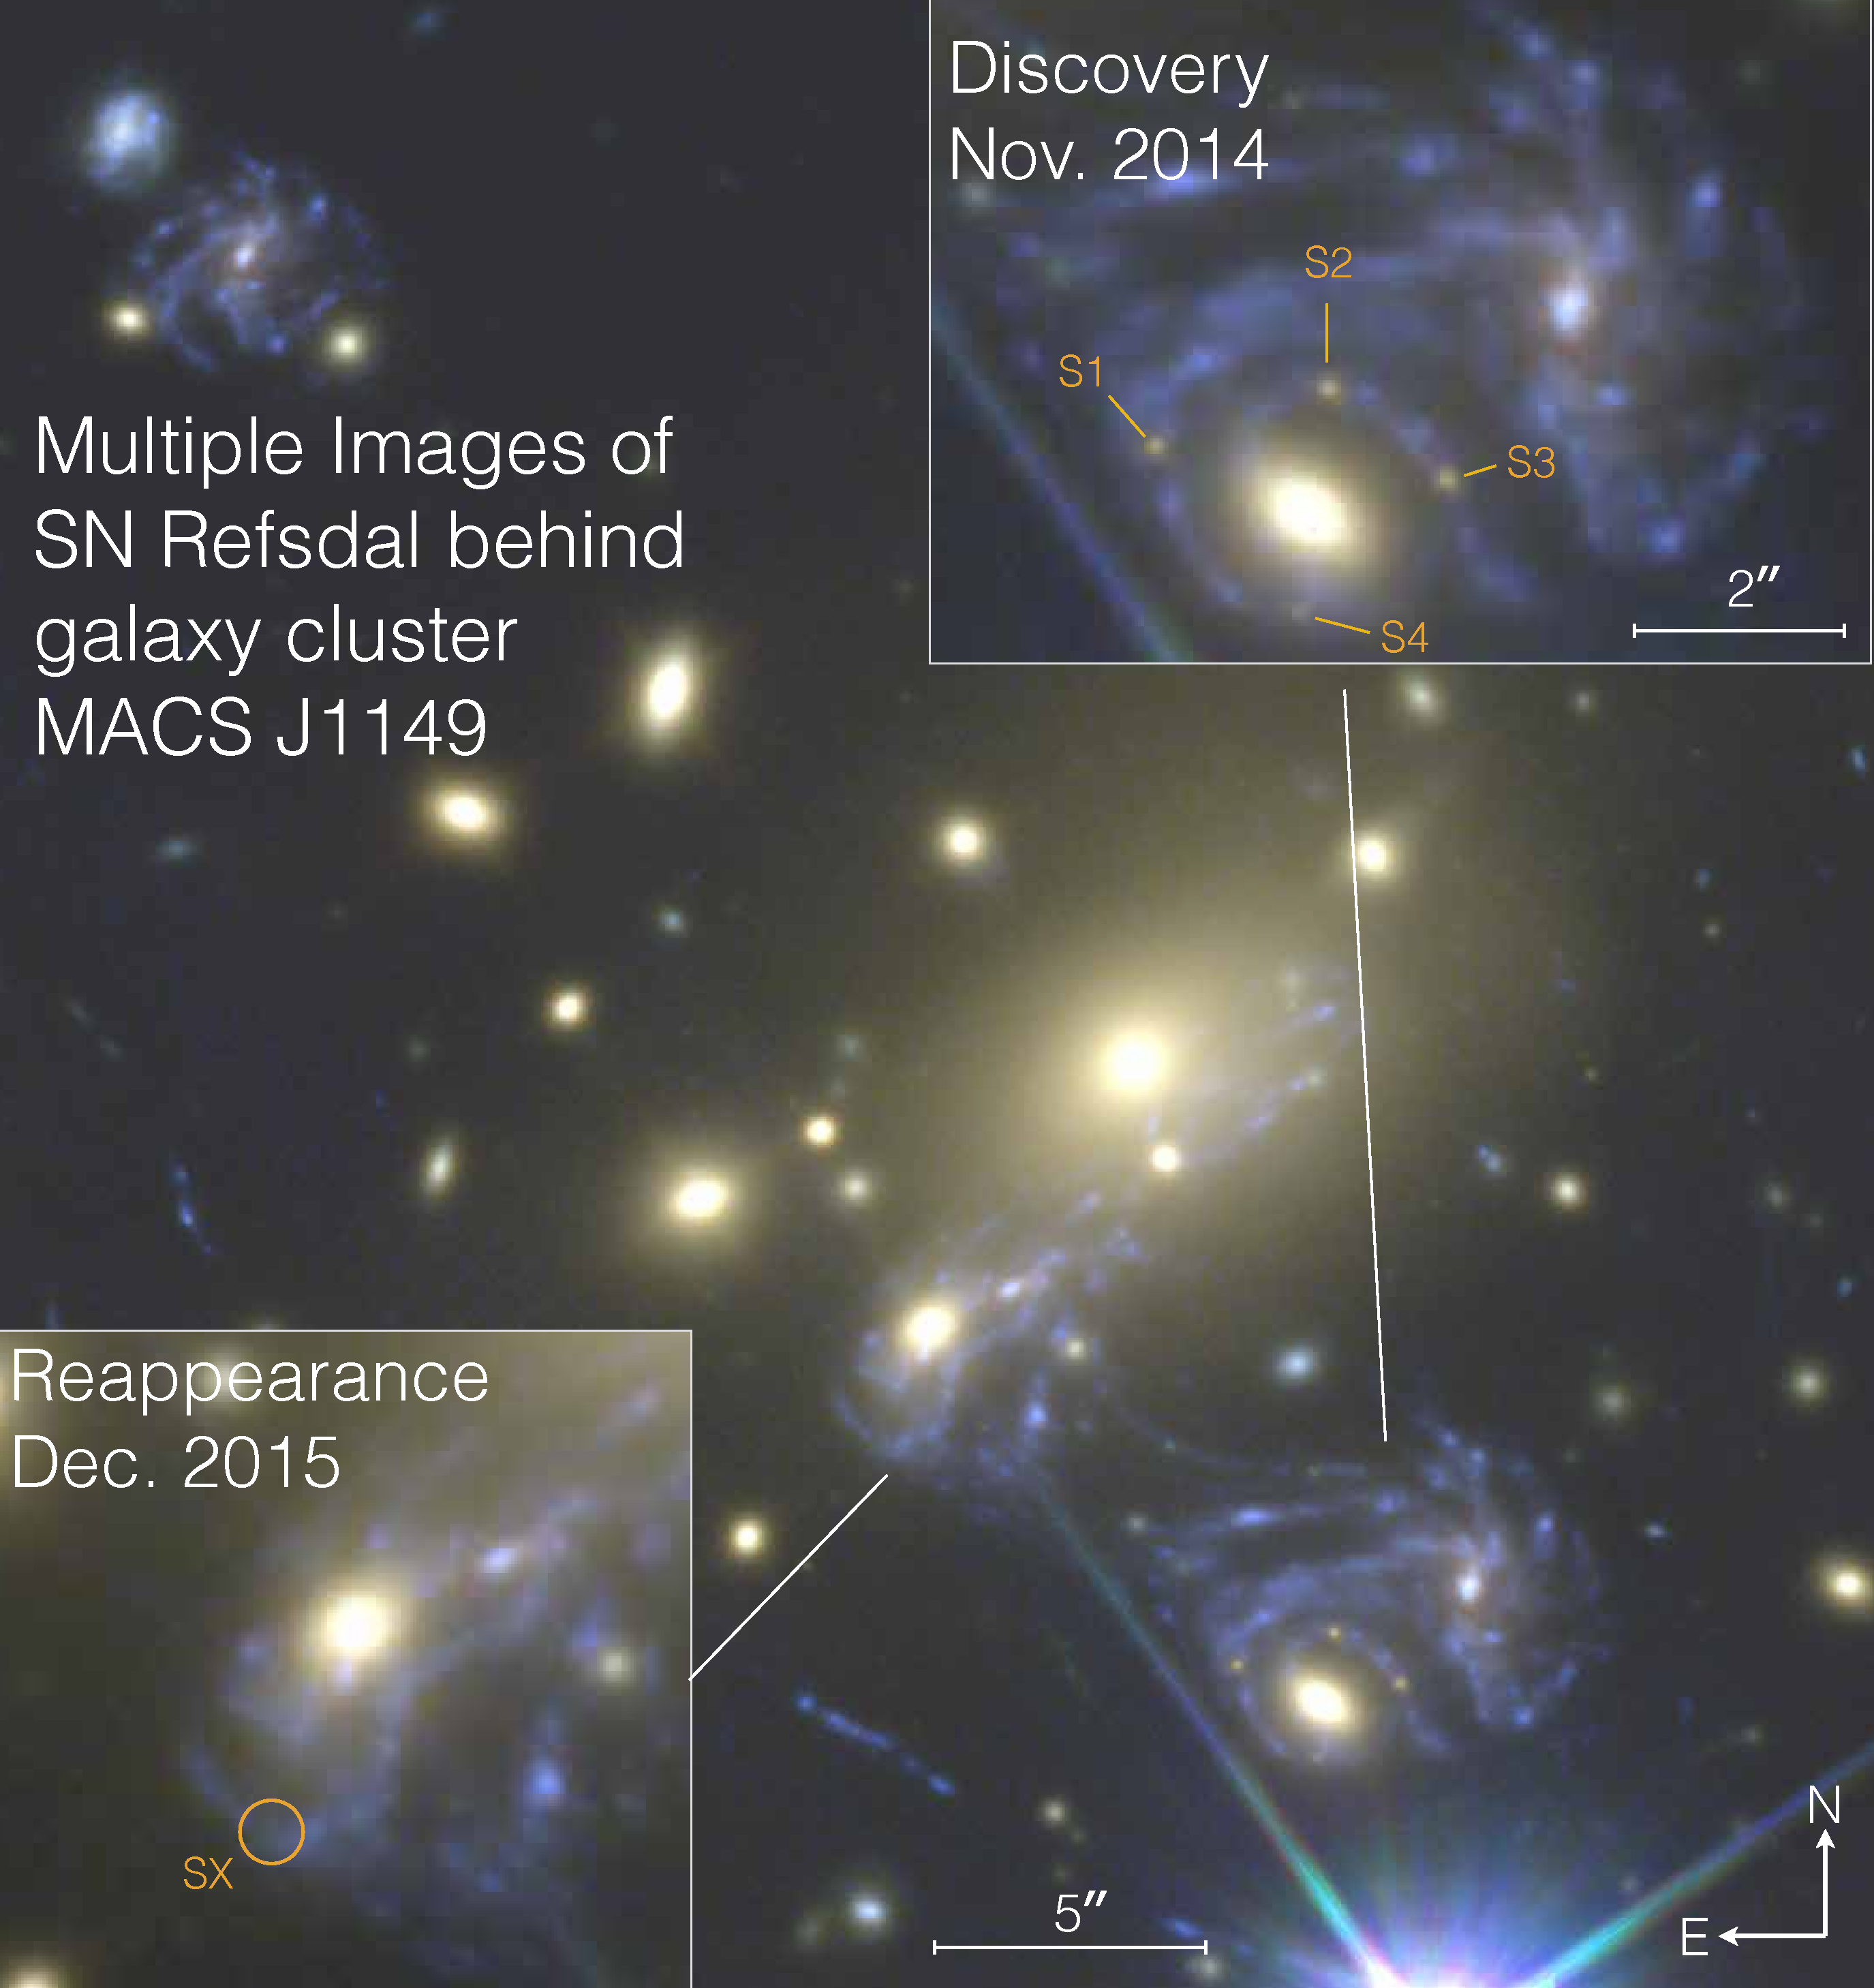
\includegraphics[height=3.6in]{FIG/refsdal_summary2}
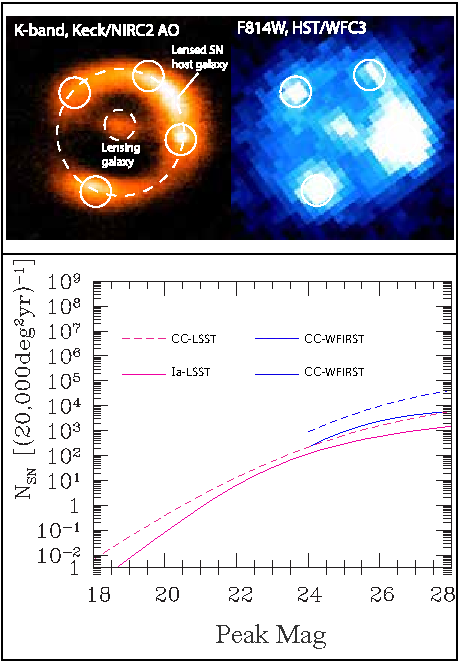
\includegraphics[height=3.6in]{FIG/lensed3}
\caption{
(A) MACS J1149.6+2223 field, showing the positions of the three primary
images of the SN Refsdal host galaxy. SN
Refsdal appears as four point sources in an Einstein Cross
configuration in the southeast spiral arm of image 1.1. (B) HST/WFC3 observation
of iPTF16geu, revealing four point sources and (C) NIR Keck observation, with the 
Einstein ring of the host galaxy clearly visible, adapted from \citet{Goobar:2016}. (D)
Expected numbers of Type Ia and Core Collapse SNe for LSST $(i_{peak,lim})$ and 
WFIRST $(H_{peak,lim})$, adapted from \citet{Oguri:2010a}.}
\end{figure}%

\forceindent The seminal work of \citet{Refsdal:1964} first showed how a
gravitationally lensed supernova (SN) resolved into multiple images
could be used as a cosmological tool.  Now, some 50 years later, HST
is playing an integral role in the long-awaited first observations of
such events (Figure 1).  HST observations caught the first
multiply-imaged SN, called ``SN Refsdal"---a core-collapse SN lensed
by both a galaxy cluster and a single galaxy (Kelly et al. 2015). This
was followed by the first multiply-imaged Type Ia SN (iPTF16geu),
resolved with HST imaging \citep{Goobar:2016}.  As the light for each
of the multiple images follows a different path through the expanding
universe and through the lensing potential, the SN images appear
delayed by hours (for galaxy-scale lenses) or years (for cluster-scale
lenses). For objects like SN Refsdal, measurement of this time delay
can be used as a precise test of cluster lens
models \citep{Treu:2015b}. For a SN like iPTF16geu, the time delay can
lead to a direct constraint on the Hubble constant that is completely
independent of the local distance ladder.

Preliminary time delay
measurements have been made, but for both SNe these are limited by the
need to include complex microlensing effects \citep{Rodney:2016,
More:2016}.  {\bf We propose to re-analyze the HST observations for
these two lensed SNe, improving the photometry and including the
significant yet previously ignored effects of microlensing.  We will
develop an open-source software package in the course of this work,
optimized for multiply-imaged SNe, that will enable precise time delay
measurements to be made for hundreds of lensed SNe expected in the
LSST/WFIRST era.}

To improve the control of systematic biases in the SN photometry, our
reanalysis will use both the \textit{PythonPhot} and
the \textit{DOLPHOT} packages. We will also measure the photometry in
single-exposure images to identify any deviations at very short
timescales, indicative of very rapid microlensing
events. \cite{Rodney:2016} measured the SN Refsdal photometry using a
static point-spread function (PSF) derived from standard
stars. However, as we know that the HST PSF does undergo subtle
variations due to telescope ``breathing," our re-analysis will use
foreground stars within the MACS1149 imaging datasets to define a
variable PSF model \textbf{The improved photometric accuracy and
precision will be critical for identifying and correcting subtle
microlensing effects.}

Microlensing refers to small-scale gravitational lensing perturbations
due to massive objects along the light path of any one image of a
multiply-imaged SN. This causes distortions in the SN light curves
that limit the precision that can be achieved in
their time delay measurements \citep{Dobler:2006}. Despite noting this significant
source of uncertainty, early analyses of SN Refsdal and iPTF16geu have
ignored microlensing due to its
complexity \citep{More:2016,Rodney:2016}. In preparing this proposal,
we have already used flexible functions to get a preliminary
measurement of microlensing for SN Refsdal (Figure 2), and it is
\textbf{clear that microlensing must be taken into account.} 
Therefore, we will analyze the effects of microlensing on a
multiply-imaged SN for the and ensure they can be accurately accounted
for in future SN analysis.

\textbf{The next decade is expected to yield observations
of tens to hundreds of multiply-imaged SNe} \citep{Oguri:2010},
yet \textbf{there is no public software package for analyzing
multiply-imaged SNe.}  A core product of this work will be an
open-source Python package for use in this and future SN
analyses. This new will be used to deliver new time delay measurements 
for SN Refsdal make , providing an important
independent check of such a measurement for the first time.

The discovery of SN iPTF16geu suggests that the \textbf{rate of
strongly lensed Type Ia SNe is likely much higher than previously
thought}, with implications for our constraints on $H_0$, the study of
galaxy sub-structures, and tests of theories of modified gravity
\citep{Goobar:2016,More:2016}. If the number of lensed Type
Ia SNe observed in the LSST/WFIRST era follows these predictions, then
it will be essential to have a publicly available, standardized tool
in place for accurate time delay and magnification
measurements. Reanalysis of these two lensed SNe offers a unique
chance to develop the tools necessary for analyzing many new lensed
SNe in the coming years, finally realizing the 50-year promise of
using lensed SNe as a new cosmological probe.

\begin{figure}[p]
\centering
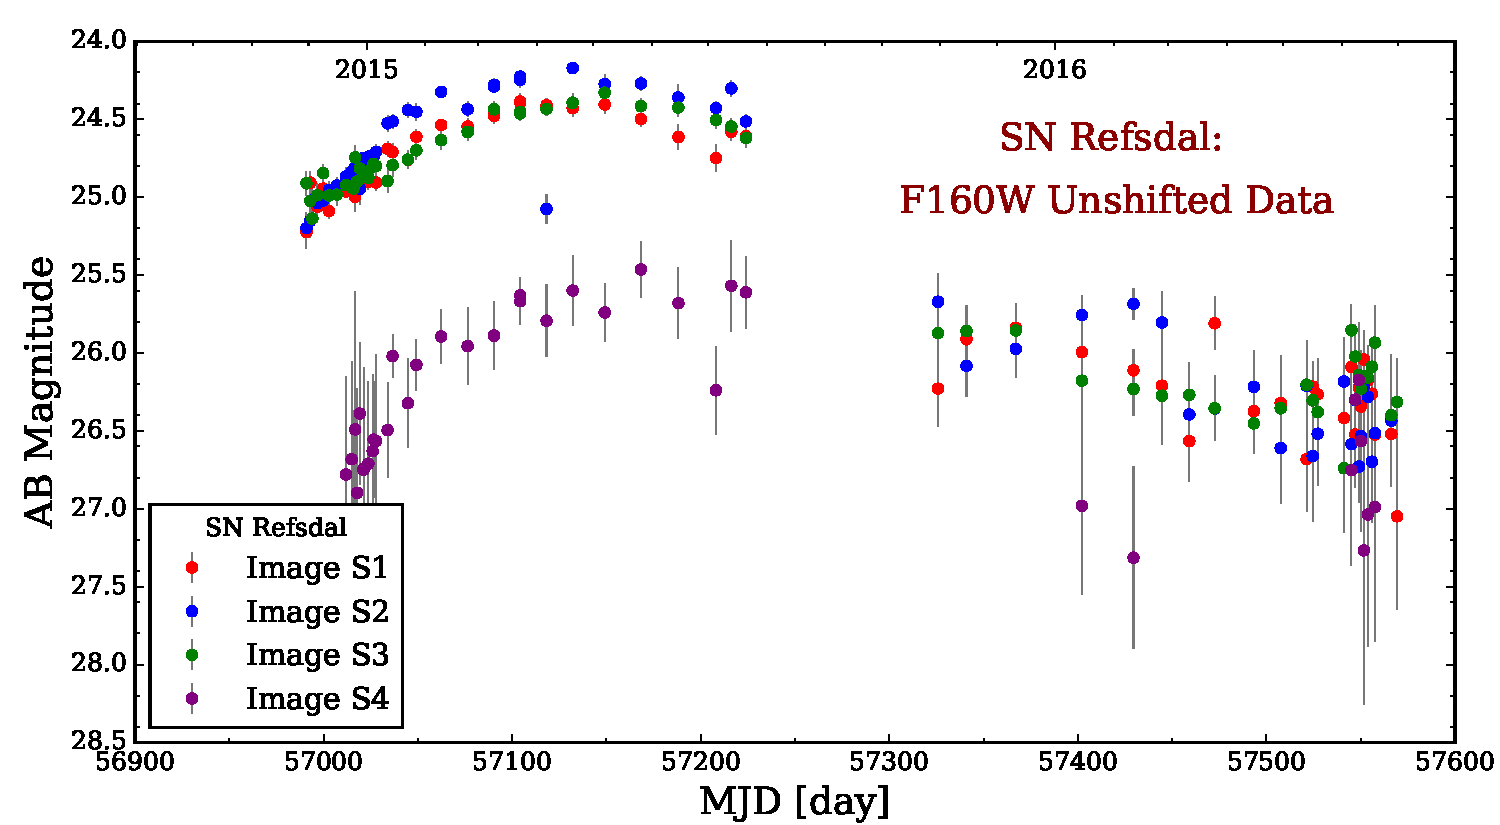
\includegraphics[width=.7\textwidth]{FIG/points_plot_2017.pdf}
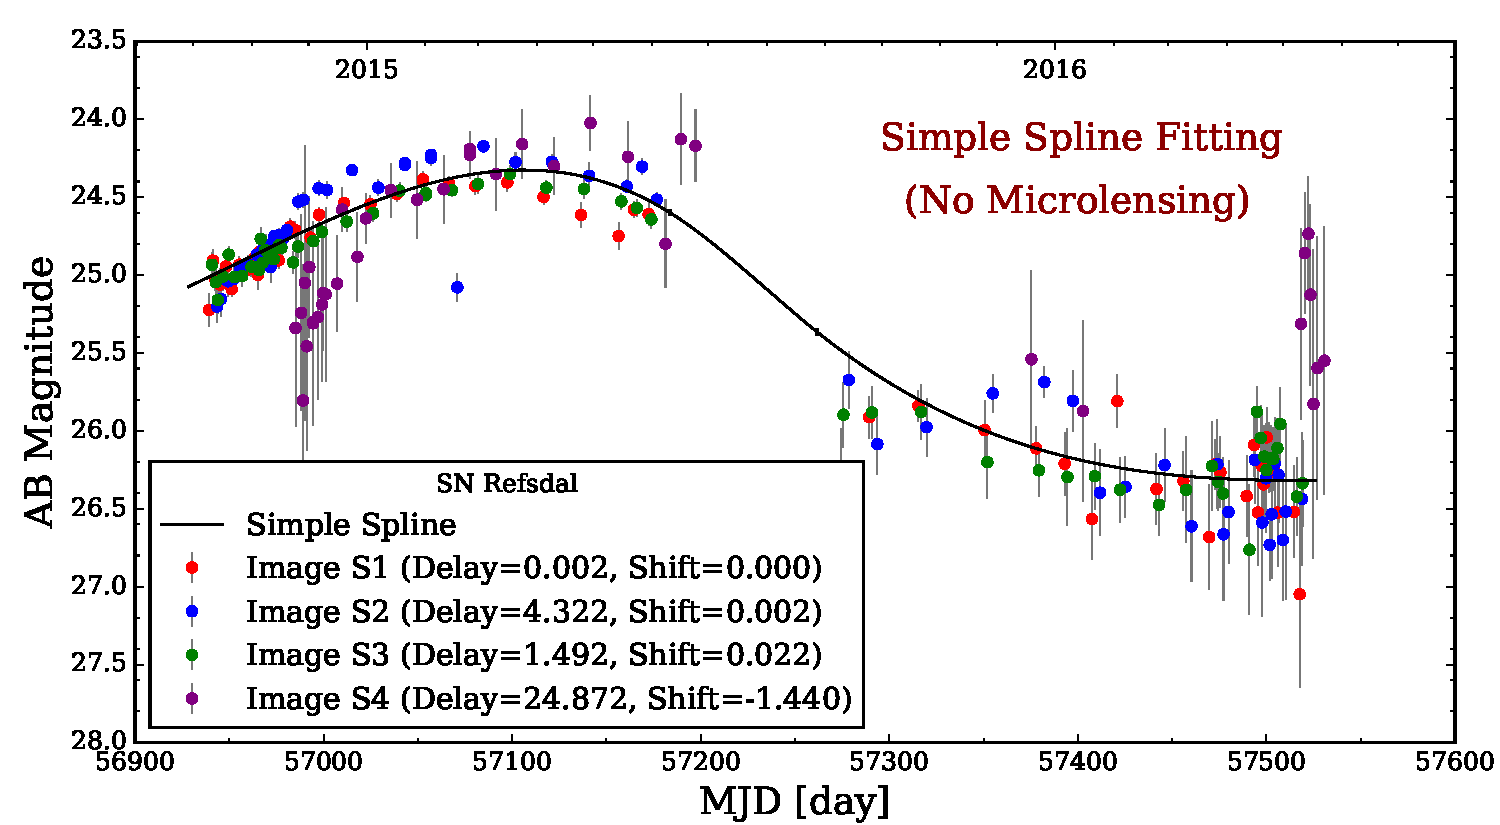
\includegraphics[width=.7\textwidth]{FIG/refs_plot_2017.pdf}
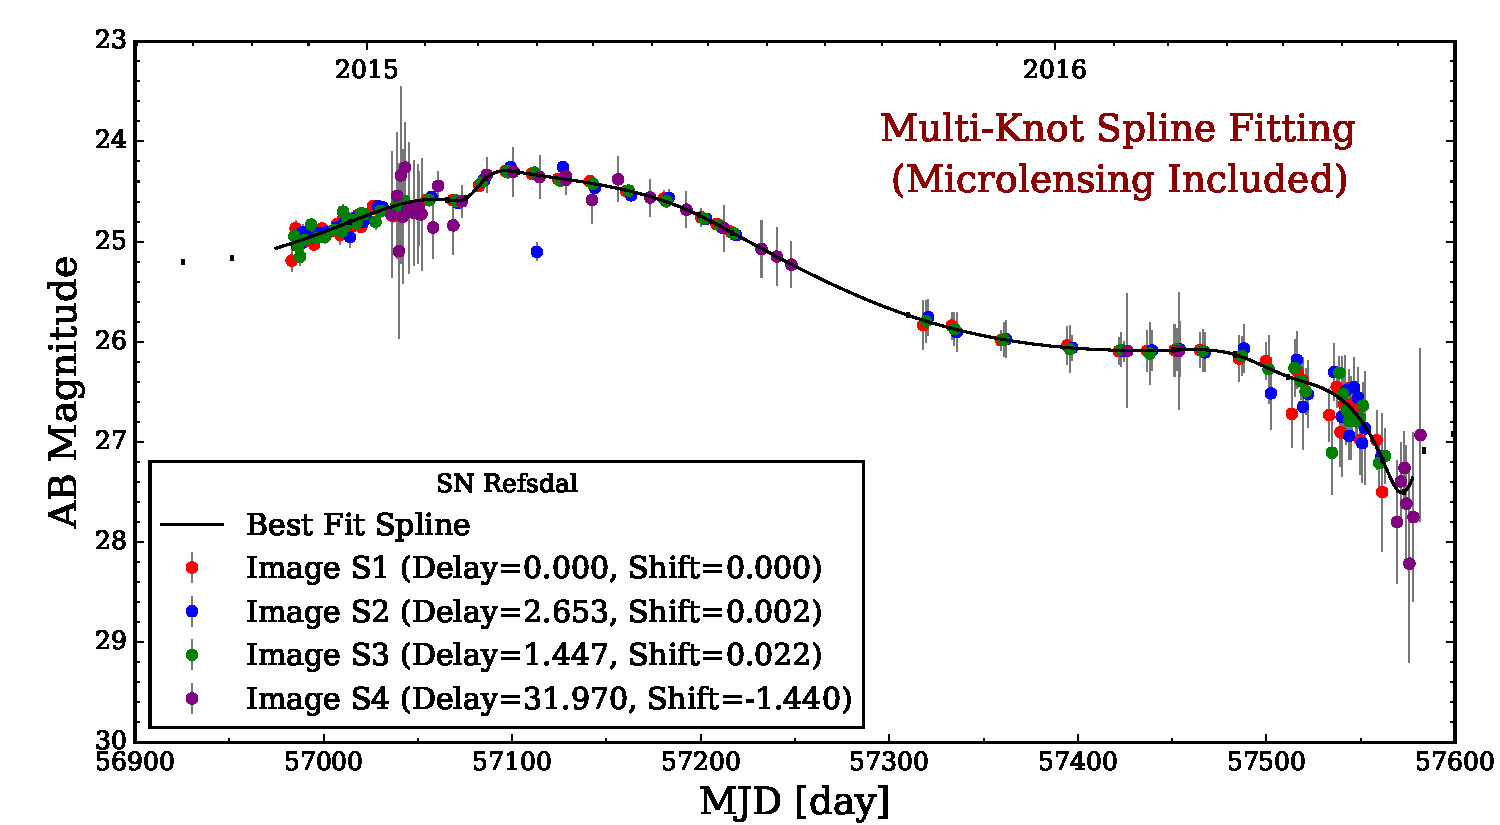
\includegraphics[width=.7\textwidth]{FIG/spline_plot_2017.pdf}
\caption{(Top) HST F160W data representing the four images of SN
Refsdal (Figure 1A), with no lensing or time shifts. (Middle) Method of
fitting the SN Refsdal light curves from Rodney et al. 2016, which did
not consider microlensing effects. (Bottom) Preliminary results from 
this work using a multi-knot spline to fit the data. This method 
includes microlensing effects, which leads to a slight adjustment in 
time delay measurements. }
\end{figure}

\bigskip
